%%%%%%%%%%%%%%%%%%%%%%%%%%%%%%%%%%%%%%%%%%%%%%%%%%%%%%%%%%%%%%%%%%%%%
% LaTeX Template: Project Titlepage Modified (v 0.1) by rcx
%
% Original Source: http://www.howtotex.com
% Date: February 2014
% 
% This is a title page template which be used for articles & reports.
% 
% This is the modified version of the original Latex template from
% aforementioned website.
% 
%%%%%%%%%%%%%%%%%%%%%%%%%%%%%%%%%%%%%%%%%%%%%%%%%%%%%%%%%%%%%%%%%%%%%%

\documentclass[12pt]{report}
\usepackage[a4paper]{geometry}
\usepackage[myheadings]{fullpage}
\usepackage{fancyhdr}
\usepackage{lastpage}
\usepackage{graphicx, wrapfig, subcaption, setspace, booktabs}
\usepackage[T1]{fontenc}
\usepackage[font=small, labelfont=bf]{caption}
\usepackage{fourier}
\usepackage[protrusion=true, expansion=true]{microtype}
\usepackage[english]{babel}
\usepackage{sectsty}
\usepackage{url}
\usepackage{amsmath}
\usepackage{upgreek}
\usepackage{comment}

\newcommand{\HRule}[1]{\rule{\linewidth}{#1}}
\onehalfspacing
\setcounter{tocdepth}{5}
\setcounter{secnumdepth}{5}

%-------------------------------------------------------------------------------
% HEADER & FOOTER
%-------------------------------------------------------------------------------
\pagestyle{fancy}
\fancyhf{}
\setlength\headheight{15pt}
\fancyfoot[R]{Page \thepage\ of \pageref{LastPage}}
%-------------------------------------------------------------------------------
% TITLE PAGE
%-------------------------------------------------------------------------------

\begin{document}

\title{ \normalsize \textsc{SC42025 Filtering and Identification}
		\\ [2.0cm]
		\HRule{0.5pt} \\
		\LARGE \textbf{\uppercase{Turbulence Modeling for Adaptive Optics}}
		\HRule{2pt} \\ [0.5cm]
		\normalsize %\today
		\vspace*{5\baselineskip}}

%\date{}

\author{
		Aniket Ashwin Samant, Snehal Jauhri \\
		(Student IDs: 4838866, 4772202) \\ 
 \\ }

\maketitle
\tableofcontents
\newpage

%-------------------------------------------------------------------------------
% Section title formatting
\sectionfont{\scshape}
%-------------------------------------------------------------------------------

%-------------------------------------------------------------------------------
% BODY
%-------------------------------------------------------------------------------

\section*{Introduction}

This assignment deals with modeling an \textit{Adaptive Optics} (AO) system in which three different data-driven turbulence modeling methods are used to achieve optimal control performances, viz.
\begin{itemize}
	\item a random-walk process
	\item a Vector-Auto-Regressive model
	\item a stochastic state-space model
\end{itemize}

Each model has some questions associated with it, and we solve them in chronological sequence taking one model at a time.


\section*{1. Random Walk Model}
\addcontentsline{toc}{section}{Random Walk Model}

We know from the assignment's equation (2) that:

\begin{equation*}
	s_{o}(k) = G\phi(k) + e(k)
\end{equation*}

We have the values of the wavefront sensor data in open-loop, $s_{o}(k)$, and also the value of the matrix \textit{G}. To compute the value of $\hat\phi(k)$, given no prior information on it, we follow the linear least-squares approach:

First, we determine whether the matrix G is full-rank or not. We load the \textit{systemMatrices.mat} file which contains the matrix G, and then run the \textit{rank} command in MATLAB to get a rank value of \textbf{47}, which is less than \textit{min(number of rows, number of columns)} of G. Thus, we need to employ a linear least-squares method that doesn't assume the matrix G to be full-rank.

We know that there are multiple solutions to this problem, and for uniqueness we go with one such that the optimal solution, $\hat\phi(k)$, has a minimal 2-norm, thus leading to the original linear least-squares problem being reformulated as:

$\underset{\phi(k) \in \Gamma}{min} \, \|\phi(k)\|_{2}^{2}$ \space	with \space	$\Gamma = \left\{ \phi(k) : \phi(k) = arg \, \underset{z}{min} \| Gz - s_{o}(k)\|_{2}^{2}\right\}$
\\
By performing an SVD operation on the matrix G, we obtain:

\begin{equation*}
G = \begin{bmatrix}
U_{1} & U_{2}
\end{bmatrix}\begin{bmatrix}
\Sigma & 0 \\
0 & 0
\end{bmatrix}
\begin{bmatrix}
V_{1}^{T} \\
V_{2}^{T}
\end{bmatrix}
= U_{1}\Sigma V_{1}^{T}
\end{equation*}

Here, $\Sigma \in \Re^{47x47}$ is non-singular, by the definition of SVD. 

Now, let us define a partitioned vector,

\begin{equation*}
\begin{bmatrix}
\xi_{1} \\
\xi_{2}
\end{bmatrix}
=
\begin{bmatrix}
V_{1}^{T} \\
V_{2}^{T}
\end{bmatrix}z
\end{equation*}

Thus, our problem becomes:

$\underset{\xi_{1}}{min} \| U_{1}\Sigma\xi_{1}z - s_{o}(k)\|_{2}^{2}$

We get $\hat\xi_{1} = \Sigma^{-1}U_{1}^{T}s_{o}(k)$, since $\Sigma$ is a non-singular matrix. $\xi_{2}$ has no effect on the above expression and can be chosen arbitrarily. Thus, we get the optimal solution,
\begin{equation*}
\hat{z} = \begin{bmatrix}
V_{1} & V_{2}
\end{bmatrix}
\begin{bmatrix}
\hat\xi_{1} \\
\hat\xi_{2}
\end{bmatrix}
= V_{1}\Sigma^{-1}U_{1}^{T}s_{o}(k) + V_{2}\hat\xi_{2}
\end{equation*}

Since we're choosing a vector $\phi(k)$ with the smallest 2-norm, and $V_{1}^{T}V_{2} = 0$ we get:

$\|\phi(k)\|_{2}^{2} = \| V_{1}\Sigma^{-1}U_{1}^{T}s_{o}(k)\|_{2}^{2} + \| V_{2}\hat\xi_{2} \|_{2}^{2}$

As we're minimizing the norm, we take $\hat\xi_{2} = 0$ and we finally get the value of $\hat\phi(k)$ to be:
\begin{equation*}
\mathbf{\hat\phi(k) = V_{1}\Sigma^{-1}U_{1}^{T}s_{o}(k)}
\end{equation*}

\subsection*{Question 2}

We are provided with some prior information about the wavefront, viz.:

\begin{itemize}
	\item E[$\phi$(k)] = 0
	\item E[$\phi(k)\phi(k)^T$] = $C_{\phi}(0)$
	\item noise variance = $\sigma_{e}^{2}$
\end{itemize}
  
Based on equation (8) from the assignment, we approximate the value of $C_{\phi}(0)$ as:
\begin{equation}\label{eq:cPhi}
C_{\phi}(0) = \frac{1}{N}\sum_{i=1}^{N}\phi(i)\phi(i)^T
\end{equation}

We have the data necessary to formulate our problem of determining $\phi(k)$ as a stochastic linear least-squares problem, and hence we define our linear estimator $\tilde{\phi}(k)$ accordingly:

\begin{equation*}
	\tilde{\phi}(k) = \begin{bmatrix}
	M & N
	\end{bmatrix}
	\begin{bmatrix}
	s_{o}(k) \\
	E[\phi(k)]
	\end{bmatrix}
\end{equation*}  

such that E$\left[(\tilde{\phi}(k)- \phi(k))(\tilde{\phi}(k)- \phi(k))^T\right]$ is minimized and E[$\tilde{\phi}(k)$] = E[$\phi(k)$] = 0
\\\\
Thus, from the assignment's equation (2), based on $s_{o}(k)$'s expression, we can say,

\begin{equation*}
	\tilde{\phi}(k) = MG\phi(k) + Me(k) + NE\left[\phi(k)\right]
\end{equation*}

Since E[$\tilde{\phi}(k)$] = E[$\phi(k)$] = 0, we have:

\begin{equation*}
\tilde{\phi}(k) = MG\phi(k) + Me(k)
\end{equation*}

Furthermore,

\begin{equation*}
\phi(k) - \tilde{\phi}(k) = (I - MG)\phi(k) - Me(k)
\end{equation*}

Thus, the covariance of the above expression is computed as:

\begin{equation*}
E\left[\left(\phi(k) - \tilde{\phi}(k)\right)\left(\phi(k) - \tilde{\phi}(k)\right)^{T}\right] = E\left[\left((I - MG)\phi(k) - Me(k)\right)\left((I - MG)\phi(k) - Me(k)\right)^{T}\right]
\end{equation*}

On expanding the right side of the equation and taking the error e(k) to be uncorrelated with the wavefront vector $\phi(k)$, and based on the statistical data provided to us, we get the following expression:

\begin{equation*}
E\left[\left(\phi(k) - \tilde{\phi}(k)\right)\left(\phi(k) - \tilde{\phi}(k)\right)^{T}\right] = (I - MG)C_{\phi}(0)(I - MG)^{T} + M\sigma_{e}^{2}IM^{T}
\end{equation*}

On further factorization, using the Schur complement of the factorized version, and the application of the "completion of squares" argument to the resulting equation, we get the optimum value of the matrix M that minimizes the covariance expression as:

\begin{equation*}
	M = C_{\phi}(0)G^{T}(GC_{\phi}(0)G^{T} + \sigma^{2}I)^{-1}
\end{equation*}

(A point to note here: the term in brackets is invertible since $C_{\phi}(0)$ is a positive definite matrix and $\sigma^{2}I$ is non-singular)

Accordingly, we also get the optimum estimate of the wavefront vector,

\begin{equation*}
\hat\phi(k|k) = C_{\phi}(0)G^{T}(GC_{\phi}(0)G^{T} + \sigma_{e}^{2}I)^{-1}s_{o}(k)
\end{equation*}

\paragraph*{}
\textit{For questions 3 to 5, we assume E[$\epsilon$(k)] = 0 and E[$\epsilon(k)\epsilon(k)^T$] = $C_{\phi}(0)$}

\subsection*{Question 3}

Now, we consider the closed-loop system, and proceed to derive a UMVE of $\epsilon(k)$ using the given measurement set s(k).
As in the previous question, we are provided with some prior information about the wavefront, viz.:

\begin{itemize}
	\item E[$\epsilon(k)$] = 0
	\item E$\left[\epsilon(k)\epsilon(k)^T\right]$ = $C_{\phi}(0)$
	\item noise variance = $\sigma_{e}^{2}$
\end{itemize}

We can clearly see that the equations (2) and (5) in the given assignment are similar, and we are told that the statistical data (the wavefront's and noise's mean and covariance values) are the same. Hence, as in the previous question, the optimum estimate of the wavefront vector is quite similar in the closed-loop system, and the only difference is in the value of the output vector, which in this case will be the closed-loop slope vector s(k):

\begin{equation*}
\hat\epsilon(k|k) = C_{\phi}(0)G^{T}(GC_{\phi}(0)G^{T} + \sigma_{e}^{2}I)^{-1}s(k)
\end{equation*}

\subsection*{Question 4}

In this question, we make use of the random walk model represented by equation (9) in the assignment.

We know that:

\begin{equation*}
\begin{aligned}
&\epsilon(k) = \phi(k) - Hu(k-1) \\
&\implies \phi(k) = \epsilon(k) + Hu(k-1) \\
&\implies \phi(k+1) = \epsilon(k+1) + Hu(k)
\end{aligned}
\end{equation*}

From the random walk model, we can relate $\phi(k)$ and $\phi(k+1)$, and substituting the above expressions respectively yields:

\begin{equation*}
\epsilon(k+1) + Hu(k) = \epsilon(k) + Hu(k-1) + \eta(k)
\end{equation*}

If we consider $\hat\epsilon(k|k)$ to be the current optimal estimate, we know that the optimal one-step ahead prediction should not be stochastic in nature, and must be estimated based on the current optimal estimate. Based on the above equation, we can thus say,

\begin{equation}\label{eq:ques4}
\hat\epsilon(k+1|k) = \hat\epsilon(k|k) + Hu(k-1) - Hu(k)
\end{equation}

\subsection*{Question 5}

We denote $\delta u(k) := u(k) - u(k-1)$. We know from the previous question's equation ~\ref{eq:ques4} that:

\begin{equation*}
\hat\epsilon(k+1|k) = \hat\epsilon(k|k) - H\delta u(k)
\end{equation*}

Thus, the minimization problem as described in the assignment's equation (6) can be reformulated as:

\begin{equation*}
	\underset{\delta u(k)}{min} \, \|\hat\epsilon(k|k) - H\delta u(k)\|_{2}^{2}
\end{equation*}

This is clearly a linear least-squares problem, and we know from running the \textit{rank} command on the matrix H that it is full-rank. Hence, we can say that the optimal increment, $\hat\delta u(k)$ for minimizing the 2-norm is:

\begin{equation*}
\hat\delta u(k) = (H^{T}H)^{-1}H^{T}\hat\epsilon(k|k)
\end{equation*}

We computed the expression for $\hat\epsilon(k|k)$ in question 3, and substituting the expression in the above equation yields the value of $\hat\delta u(k)$ as:

\begin{equation}\label{eq:delta_uk}
\hat\delta u(k) = (H^{T}H)^{-1}H^{T}C_{\phi}(0)G^{T}(GC_{\phi}(0)G^{T} + \sigma_{e}^{2}I)^{-1}s(k)
\end{equation}

\begin{comment}
Moreover, since H is invertible, we can further simplify the expression as:

\begin{equation}\label{eq:delta_uk}
\hat\delta u(k) = H^{-1}C_{\phi}(0)G^{T}(GC_{\phi}(0)G^{T} + \sigma_{e}^{2}I)^{-1}s(k)
\end{equation}
\end{comment}

\subsection*{Question 6}

Given all the data, we compute the values for u(k) recursively based on the values of u(k-1) as defined by the relation in equation \ref{eq:delta_uk}. We take u(1) to be 0, since we assume that for the first iteration, there's no input actuation applied through the deformable mirror. Accordingly, we get:

\begin{equation*}
\epsilon(1) = \phi_{sim}(1)
\end{equation*}

Moreover, since we're provided with $\phi_{sim}$ values but not the values for the actual slope measurements s(k), we compute s(k) as: 

\begin{equation*}
s(k) = G\epsilon(k) + \sigma_{e}*randn(N_{s},1) 
\end{equation*}

where \texttt{randn()} is a MATLAB function used for generating a normally distributed random noise vector.
This s(k) is used in the computation of the optimum u(k) value.
We iterate over all the time samples to get the u(k) matrix for all input vectors, and once we have these values, we can calculate the $\epsilon$ matrix for all time samples based on: 

\begin{equation*}
\epsilon(k) = \phi(k) - Hu(k-1) 
\end{equation*}

We apply the correction process of subtracting the mean vector from $\epsilon(k)$ and then calculate the variance of the vector. The variance for each time sample is calculated accordingly and the average variance of all time samples is returned by the function \texttt{AOloopRW()}.

\subsection*{Question 7}

We compare the variance values returned by the random-walk model-based control design and the open-loop case (in which no control is applied). The variance returned by the former is around a value of 6.5 whereas the latter's returned value is around 22. We can clearly see a reduction in the variance of $\epsilon(k)$ values after controlling the residual wavefront using the DM.

The VAF is calculated based on another function, \texttt{VAF\_RW} in which the $\phi(k+1|k)$ values are compared against $\phi_{sim}(k+1)$ values (after taking into consideration the mean value subtraction as performed in Question 6). The value returned is around 70\%.

\newpage
\section*{2. VAR Model of Order 1}
\addcontentsline{toc}{section}{VAR Model of Order 1}

We are provided with a VAR model represented by:

\begin{equation}\label{eq:var_eqn}
	\phi(k+1) = A\phi(k) + w(k)
\end{equation}

We have the following information provided to us to demonstrate that w(k) is uncorrelated with the measurement noise and the wavefront:
\begin{itemize}
\item $E\left[w(k)e(k)^{T}\right] = 0$
\item $E\left[w(k)\phi(k)^{T}\right] = 0$
\end{itemize}

We are also provided with statistical information about w(k): w(k) $\sim \mathcal{N}(0, C_{w})$

\subsection*{Question 1}

We have the following data:

\begin{itemize}
	\item $C_{\phi}(0) = E\left[\phi(k)\phi(k)^{T}\right]$
	\item $C_{\phi}(1) = E\left[\phi(k+1)\phi(k)^{T}\right]$
\end{itemize}

Multiplying equation \ref{eq:var_eqn} with $\phi(k)^{T}$ on both sides yields:

\begin{equation*}
\phi(k+1)\phi(k)^{T} = A\phi(k)\phi(k)^{T} + w(k)\phi(k)^{T}
\end{equation*}

Further, on taking the expectation:

\begin{equation*}
E\left[\phi(k+1)\phi(k)^{T}\right] = E\left[A\phi(k)\phi(k)^{T}\right] + E\left[w(k)\phi(k)^{T}\right]
\end{equation*}

Thus, we get the relation:

\begin{equation*}
	C_{\phi}(1) = AC_{\phi}(0)
\end{equation*}

and hence we calculate:
\begin{equation*}
	A = C_{\phi}(1)C_{\phi}(0)^{-1}
\end{equation*}


\subsection*{Question 2}

We make an assumption here that $\phi(k)$ is a WSS signal.

Multiplying equation \ref{eq:var_eqn} with $w(k)^{T}$ on both sides, and then taking the resulting expectation yields:

\begin{equation*}
E\left[\phi(k+1)w(k)^{T}\right] = E\left[A\phi(k)w(k)^{T}\right] + E\left[w(k)w(k)^{T}\right]
\end{equation*} 

Based on the data we have, we get the following relation based on the above equation:

\begin{equation*}
	E\left[\phi(k+1)w(k)^{T}\right] = C_{w}
\end{equation*}

Taking the transpose of equation \ref{eq:var_eqn}, and multiplying with $\phi(k+1)$ on both sides, we get: 

\begin{equation*}
E\left[\phi(k+1)\phi(k+1)^{T}\right] = E\left[A\phi(k+1)\phi(k)^{T}\right] + E\left[\phi(k+1)w(k)^{T}\right]
\end{equation*} 

Since we have assumed $\phi(k)$ to be WSS, we can say that:\newline
$E\left[\phi(k+1)\phi(k+1)^{T}\right] = E\left[\phi(k)\phi(k)^{T}\right] = C_{\phi}(0)$ 

And we know from the previous question that $C_{\phi}(1) = AC_{\phi}(0)$\newline
Thus,

\begin{equation*}
\begin{aligned}
C_{\phi}(0) = AC_{\phi}(1) + C_{w}\\
\implies C_{\phi}(0) = A^2C_{\phi}(0) + C_{w}
\end{aligned}
\end{equation*}

So we derive the following relationship:

\begin{equation*}
C_{w} = (I-A^2)C_{\phi}(0)
\end{equation*} 

\subsection*{Question 3}

We need to formulate a state-space model with $\epsilon(k)$ being the state vector and s(k) being the output.

Based on equation (4) from the assignment, we can write:

\begin{equation*}
\begin{aligned}
\phi(k) = \epsilon(k) + Hu(k-1)\\
\implies \phi(k+1) = \epsilon(k+1) + Hu(k)
\end{aligned}
\end{equation*} 

Substituting this expression for $\phi(k)$ in equation (10), we get:

\begin{equation*}
\begin{aligned}
\epsilon(k+1) + Hu(k) = A\epsilon(k) + AHu(k-1) + w(k)\\
\implies \epsilon(k+1) = A\epsilon(k) + AHu(k-1) - Hu(k) + w(k)
\end{aligned}
\end{equation*} 

Combining the above relation with equation (5) from the assignment, we have the following state-space model as required:

\begin{equation*}
\begin{aligned}
\epsilon(k+1) &= A\epsilon(k) + \xi(k) + w(k)\\
s(k) &= G\epsilon(k) + e(k)\\
&where\\
\xi(k) &= AHu(k-1) - Hu(k)
\end{aligned}
\end{equation*} 

\subsection*{Question 4}

Based on the state-space formulation from Question 3, we can express the Kalman filter in the observer form as:

\begin{equation*}
	\hat\epsilon(k+1) = (A - KG)\epsilon(k) + AHu(k-1) - Hu(k) + Ks(k)
\end{equation*}

We make use of the following DARE to compute the covariance matrix of $\epsilon(k)$, P, to which the optimal estimate of $\hat P(k+1|k)$ converges on solving the Kalman filter problem, as k $\rightarrow \infty$:

\begin{equation*}
\begin{aligned}
P &= APA^{T} + Q - (APG^{T})(GPG^{T} + R)^{-1}(APG^{T})^{T}\\
&where:\\
Q &= C_{w}\\
R &= E[v(k)v(k)^{T}]
\end{aligned}
\end{equation*}

An important point to note here is that v(k) and w(k) are taken to be uncorrelated, and the matrices A and G to be time-invariant.

Based on the P matrix calculated on solving the above Riccati equation, we compute the value of the stationary Kalman gain,

\begin{equation*}
	K = APG^{T}(GPG^{T} + R)^{-1}
\end{equation*}

\subsection*{Question 5}

The minimum unbiased variance estimate for a state $x(k+1)$ is given by the following expression, which is derived based on the conditions of the conventional Kalman filtering problem (here, we assume a stationary Kalman filter):

\begin{equation*}
\hat{x}(k+1|k) = Ky(k) + Bu(k) + (A - KC)\hat{x}(k|k-1)
\end{equation*}

Here, x(k) is the state vector, y(k) is the output, and A,B, and C are the state-space matrices. In our case, based on our LTI state-space model with $\epsilon(k)$ being the state vector, s(k) being the output vector, and A and G being the state-space matrices, we compute the expression for the optimal one step ahead prediction recursively as:

\begin{equation}\label{eq:eps_optimal}
	\hat\epsilon(k+1|k) = Ks(k) + AHu(k-1) - Hu(k) + (A - KG)\hat\epsilon(k|k-1)
\end{equation}

\subsection*{Question 6}

Based on the control law represented by equation (6) in the assignment, we need to minimize the value of $\|\hat\epsilon(k+1|k)\|_{2}^{2}$ by controlling the input values u(k). From equation \ref{eq:eps_optimal}, we know that we need to minimize the value of:

\begin{equation}
\|(Ks(k) + (A - KG)\hat\epsilon(k|k-1)) + AHu(k-1) - Hu(k) \|_{2}^{2}
\end{equation}

Let us take $\xi(k) = Hu(k) - AHu(k-1)$

In the above equation, let us denote:

$Y(k) = Ks(k) + (A - KG)\hat\epsilon(k|k-1) + AHu(k-1)$

Hence, our minimization problem becomes:

\begin{equation}
\underset{u(k)}{min} \, \| Y(k) - Hu(k) \|_{2}^{2}
\end{equation}

Knowing H to be full-rank and square, we have the linear least-squares solution,

$\hat{u}(k) = H^{-1}Y(k)$

That is to say,

\begin{equation}
\hat{u}(k) = H^{-1}(Ks(k) + (A - KG)\hat\epsilon(k|k-1)) + H^{-1}AHu(k-1)
\end{equation}

Hence the optimum input vectors can be calculated recursively.

\subsection*{Question 7}

The first function, \texttt{computeKalmanAR()} is used for calculating the values of A, $C_{w}$, and K using expressions derived previously in questions 1,2, and 4 respectively.

The function \texttt{AOloopAR()} is used for calculating the values of u(k) for which the 2-norm of $\epsilon(k+1|k)$ is minimum. It is performed using the expression derived in Question 6, and taking $\hat\epsilon(1|0)$ and u(0) to be 0.

u(k) and $\hat\epsilon(k+1|k)$ for the remaining indices can be calculated based on the recursive expressions for the two quantities. Once we have the u(k) values, the $\epsilon(k)$ values can be calculated as $\phi_{sim}(k) - Hu(k-1)$, and accordingly the average variance value can be calculated, as was done in Question (1.) 6 of the random walk model approach.

The variance value of $\epsilon$ returned by \texttt{AOloopAR()} is around 3.5.

\subsection*{Question 8}

We compare the average variance value obtained in this case as against in the random walk model's. The value is further reduced using this model, and we see that this model outperforms the random walk model in terms of minimizing the variance of the estimates.

We compute the VAF for the turbulence wavefront one step ahead predicted values as in the previous case by comparing the predicted $\hat\phi(k+1|k)$ vectors against the $\phi_{sim}(k+1)$ vectors, and obtain a value of around 83 \%.

\newpage
\section*{3. Subspace Identification}
\addcontentsline{toc}{section}{Subspace Identification}

We are provided with a turbulence state space model description with a general state vector $x$ and are tasked with finding the Matrices $A_s$, $C_s$ and the Kalman gain $K_s$ of the system in innovation form.

\begin{equation}
\begin{aligned}
x(k+1) &= A_s x(k) + K_s v(k)\\
s(k) &= C_s x(k) + v(k)
\end{aligned}
\end{equation}

We generate the identification data i.e. $s_id$ using the provided $\phi_{id}$ data.

\subsection*{Question 1}
We use the N4SID method to estimate the State matrices and the state sequence. This is to ensure that we get the matrices and the Kalman gain up to the same similarity transformation.
\\
\textbf{Data Equation:}\\
\begin{equation}
Y_{s,s,N} = O_s X_{s,N} + \uptau_{v,s} V_{s,s,N}
\end{equation}
Where $Y$,$X$ and $V$ are the Hankel Matrices and $O_s$ is the observability matrix. $\uptau$ is the Toeplitz matrix for the innovation signal.\\
\textbf{Instrumental Variable:}\\
The instrumental variable for our data equation is chosen as:\\
\begin{equation*}
Z_N = Y_{0,s,N}
\end{equation*}
This $Z_N$ thus eliminates $V_{s,s,N}$ from the data equation and gives:
\begin{equation*}
\underset{N\rightarrow \infty}{Lt} \frac{1}{N} Y_{s,s,N} Y_{o,s,N}^{T} = \underset{N\rightarrow \infty}{Lt} \frac{1}{N} O_{s} X_{s,N} Y_{o,s,N}^{T}
\end{equation*}
\\
We use an RQ factorization of the Instrumental variable for efficiency:\\
\begin{equation*}
\begin{bmatrix}
Y_{0,s,N}\\
Y_{s,s,N}\\
\end{bmatrix}
 = \begin{bmatrix}
 R_{11} & 0\\
 R_{21} & R_{22}\\
 \end{bmatrix}
 \begin{bmatrix}
 Q_1\\
 Q_2\\
 \end{bmatrix}
\end{equation*}
\\
And so,
\begin{equation}
O_s X_{s,N} \approx R_{21} R_{11}^{-1} Z_N
\end{equation}
\\
The rank of the above expression (11) is n.\\
Hence we can use this RQ approximation and take it's SVD:\\
\begin{equation*}
R_{21} R_{11}^{-1} Z_N = U_n \Sigma_n V_n^T
\end{equation*}
State sequence is hence estimated as,
\begin{equation*}
\hat{X}_{s,N} = \Sigma_n^{1/2} V_n^T
\end{equation*}
We now use this state sequence to find our State Matrices by solving the linear least squares problem:
\begin{equation*}
\|
\begin{bmatrix}
\hat{X}_{s+1,N}\\
\hat{Y}_{s,1,N-1}\\
\end{bmatrix}
- \begin{bmatrix}
A_T\\
C_T\\
\end{bmatrix}
\begin{bmatrix}
\hat{X}_{s,N-1}\\
\end{bmatrix}
\|_{F}^2
\end{equation*}
\\
We solve this problem analytically, using the general least squares solution to a problem $\| y - Fx \|_{2}^2$ which is $\hat{x} = (F^T F)^{-1}F^T y$.
\\
This completes the state estimation and computing the state matrices.
\subsection*{Question 2}
Using the results from the previous question, we can compute the co-variances of our state estimate and identification data (including cross-covariance). This is done using the residuals from our optimal state estimate and our identified state matrices:\\
\begin{equation*}
\begin{bmatrix}
\hat{W}_{s,1,N-1}\\
\hat{V}_{s,1,N-1}
\end{bmatrix}
=
\begin{bmatrix}
\hat{X}_{s+1,N}\\
\hat{Y}_{s,1,N-1}\\
\end{bmatrix}
- \begin{bmatrix}
A_T\\
C_T\\
\end{bmatrix}
\begin{bmatrix}
\hat{X}_{s,N-1}\\
\end{bmatrix}
\end{equation*}
Thus, our co-variances are computed as:\\
\begin{equation*}
\begin{bmatrix}
\hat{Q} & \hat{S}\\
\hat{S}^T & \hat{R}\\
\end{bmatrix}
=\underset{N\rightarrow \infty}{Lt}\frac{1}{N}
\begin{bmatrix}
\hat{W}_{s,1,N-1}\\
\hat{V}_{s,1,N-1}
\end{bmatrix}
\begin{bmatrix}
\hat{W}_{s,1,N-1}^T & \hat{V}_{s,1,N-1}^T\\
\end{bmatrix}
\end{equation*}
Now that we have our co-variances, we can use the solution of the stationary Kalman equation to find optimal kalman gain $K_s$. This is done by solving a Ricatti equation of the form:\\
\begin{equation*}
\hat{P} = \hat{A}_T\hat{P}\hat{A}_T^T + \hat{Q} - (\hat{S} + \hat{A}_T\hat{P}\hat{C}_T^T)(\hat{C}_T\hat{P}\hat{C}_T^T + \hat{R})^{-1}(\hat{S} + \hat{A}_T\hat{P}\hat{C}_T^T)^T
\end{equation*}
And the Kalman Gain is:\\
\begin{equation*}
\hat{K}_T = (\hat{S} + \hat{A}_T\hat{P}\hat{C}_T^T)(\hat{C}_T\hat{P}\hat{C}_T^T + \hat{R})^{-1}
\end{equation*}
This completes the computation of the Covariances and the Kalman Gain.
\subsection*{Question 3}
Now that we know our State Space matrices (lets call them $A_s$, $C_s$) and our optimal Kalman Gain ($K_s$), we can use our turbulence model to obtain optimal prediction for our next state i.e. $\hat{x}(k+1|k)$ and consequently the optimal predition for the next open loop slope $\hat{s}(k+1|k)$.\\
If the current output slope is $s(k)$, we can find the current innovation signal and hence write our prediction $\hat{x}(k+1|k)$ as:
\begin{equation}
\hat{x}(k+1|k) = A_s\hat{x}(k|k-1) + K_s(s(k) - C_s\hat{x}(k|k-1))
\end{equation}
Starting from an initial estimate $x(0)$, our Kalman implementation should eventually converse and provide a good estimate of $\hat{x}(k+1|k)$ and in turn, of $\hat{s}(k+1|k)$:
\begin{equation*}
\hat{s}(k+1|k) = C_s\hat{x}(k+1|k)
\end{equation*}
Since we need the optimal prediction of $\phi$, we can now use $\hat{s}(k+1|k)$ to find $\hat{\phi}(k+1|k)$ using the expression derived in Part 1.1 which is:
\begin{equation*}
\hat{\phi}(k+1|k) = V_{1}\Sigma^{-1}U_{1}^{T}\hat{s}(k+1|k)
\end{equation*}
where $V_{1}\Sigma^{-1}U_{1}^{T}$ represents the pseudo inverse of the matrix $G$ found using SVD.\\
We can now use this $\hat{\phi}(k+1|k)$ to arrive at an expression for the residual $\hat{\epsilon}(k+1|k)$:
\begin{equation*}
\begin{aligned}
\hat{\epsilon}(k+1|k) &= \hat{\phi}(k+1|k) - Hu(k)\\
\hat{\epsilon}(k+1|k) &= V_{1}\Sigma^{-1}U_{1}^{T}\hat{s}(k+1|k) - Hu(k)\\
\end{aligned}
\end{equation*}
So finally we get:
\begin{equation}
\hat{\epsilon}(k+1|k) = V_{1}\Sigma^{-1}U_{1}^{T}C_s\hat{x}(k+1|k) - Hu(k)
\end{equation}
\subsection*{Question 4}
The control action that minimises $\hat{\epsilon}(k+1|k)$ as in equation (13) can be found by solving the least squares problem:\\
\begin{equation*}
\|\hat{\epsilon}(k+1|k)\|^2_2 = \|V_{1}\Sigma^{-1}U_{1}^{T}C_s\hat{x}(k+1|k) - Hu(k)\|^2_2
\end{equation*}
The analytical solution looks like:\\
\begin{equation}
\hat{u}(k) = (H^T H)^{-1}H^TV_{1}\Sigma^{-1}U_{1}^{T}C_s\hat{x}(k+1|k)
\end{equation}
Hence we have found a minimising control input $u$.
\subsection*{Question 5}
\textbf{Approach:}
We ran the subspace Identification and Validation for the given datasets $\phi_{ident}$ and $\phi_{sim}$ respectively.\\
The System Identification cycle was completed multiple times for different sets of $\phi_{ident}$ and $\phi_{sim}$ to avoid overfitting any particular dataset and to arrive at reliable average variance and VAF values.\\
Matlab Implementation attached in the Appendix.

\subsection*{Question 6}
\textbf{Results:}
\begin{itemize}
	\item \textbf{Average VAF} for the estimate $\hat{\phi}(k+1|k)$ achieved through this method is \textbf{90.8295\%}. This clearly shows that the state space turbulence model, found using the Subspace Identification method, works best as compared to models in Part 1 and 2 in terms of estimating the actual wavefront $\phi$.
	\item \textbf{Average Variance} of the residual achieved through this method is \textbf{2.0329}. This displays the improved closed loop performance of our method used in Part 3 as compared to Part 1 and 2.
	\item The parameter $n$ for Subspace Identification was chosen by observing the Singular Values of the RQ approximation $R_{21} R_{11}^{-1} Z_N$ since this SVD has the same column space as the Observability matrix $O_s$. The plot for the Singular values is shown in Figure 1 below:\\
\begin{figure}[!t]
	\centering
	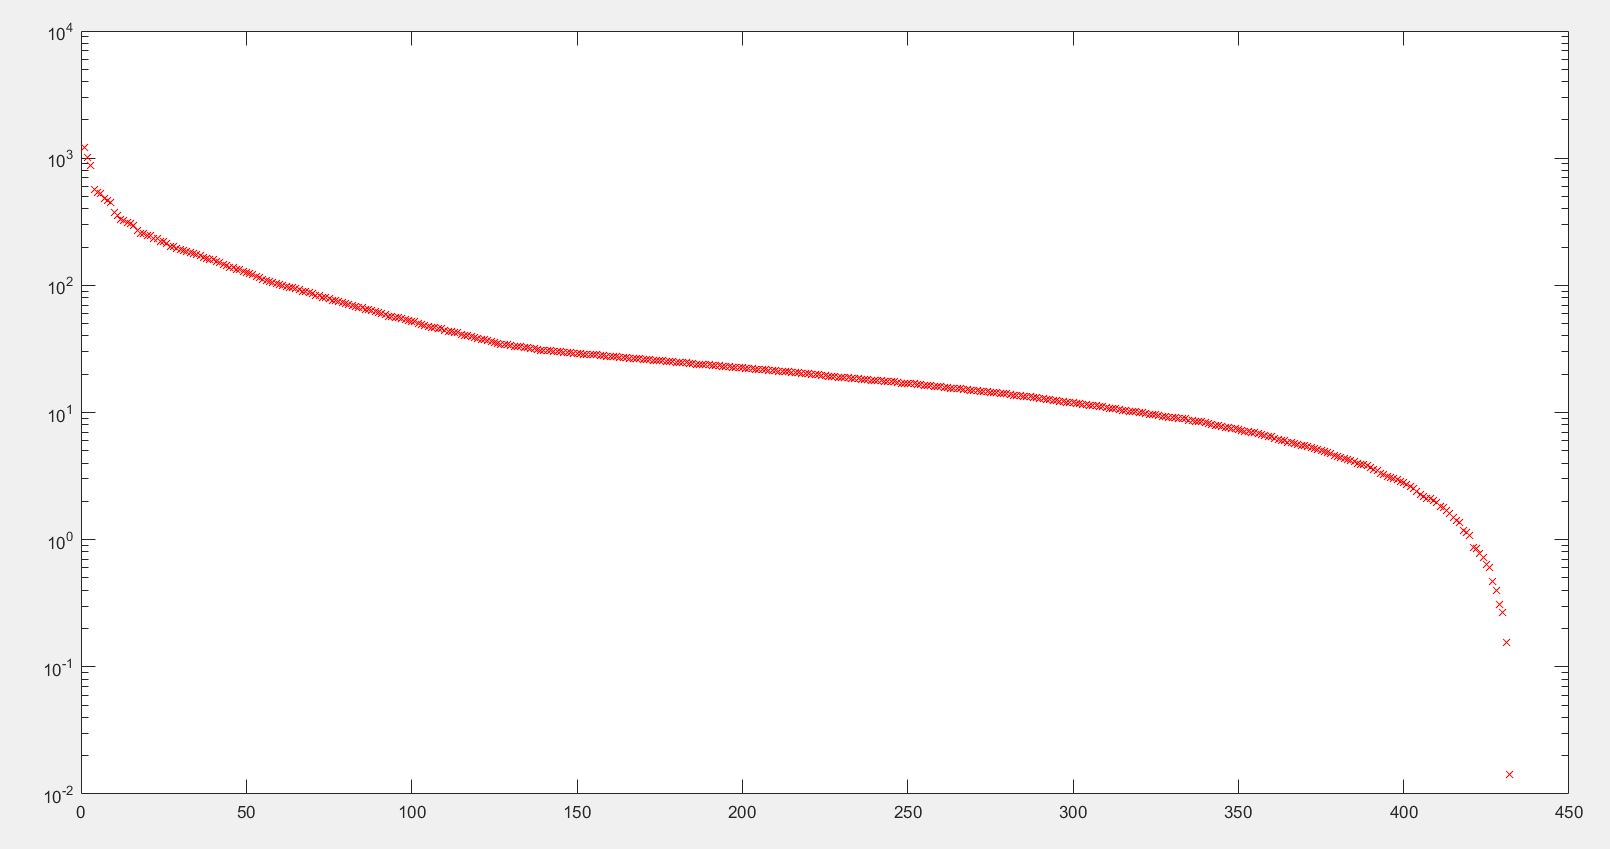
\includegraphics[width=0.9\linewidth]{SubIDSVD.JPG}
	\caption{Singular Value Distribution of $R_{21} R_{11}^{-1} Z_N$}
	\label{fig:SVD SubID}
\end{figure}
	An analysis of this distribution shows that the first 3 to 6 singular values are the most important and subsequent Singular values are quite close to each other in terms of magnitude. Thus, a mimimum order of 6 is essential. While there are improvements on choosing a larger order n, we get diminishing returns. Another consideration for $n$ is the amount of computation that would be required for the turbulence model identification and validation when choosing a large $n$.\\
	After experimenting  with different identification datasets and validating them, we arrived at an optimum value of \textbf{$n = 60$}. This captures most of the information from the dataset while not being too large for computation and achieves good results for Variance and VAF
	\item The parameter $s$ for Subspace Identification was chosen based on the law: $2p^2s > n$, where $p$ is the number of lenslets in the Shack-Hartmann sensor and so $(p+1)^2$ is the dimension of a wavefront $\phi$. In principle, this condition ensures that $s$ is large enough to identify an $n^{th}$ order system and satisfies rank conditions.\\
	After experimenting  with different identification datasets and validating them, we arrived at an optimum value of $s = 6$. We noticed that using a large value of $s$ i.e. a value close to $n$ leads to worse performance. Hence s was kept small while still satisfying the law: $2p^2s > n$.
	\item The parameters $N_{val}$ and $N_{id}$ were not used since we performed our validation on the simulation dataset $\phi_{sim}$ in the 'AOlooSID' function.
	
\end{itemize}

\newpage
\section*{4. Critical Thinking}
\addcontentsline{toc}{section}{Critical Thinking}

\subsection*{Question 1}

In this question, we make use of a slightly different version of the random walk model presented in Section 1, with the control law requiring the minimization of the residual slopes s(k+1) instead of $\epsilon(k+1)$.

We know from equation (5) of the assignment that:

\begin{equation*}
\hat{s}(k+1|k) = G\hat\epsilon(k+1|k)
\end{equation*}

Writing $\hat\epsilon(k+1|k) = \hat\phi(k+1|k) - Hu(k)$, we obtain the relation:

\begin{equation*}
\hat{s}(k+1|k) = G\hat\phi(k+1|k) - GHu(k)
\end{equation*}

Since we are making use of the random walk model as described by equation (9), we know the relation: $\hat\phi(k+1|k) = \hat\phi(k|k)$

Moreover, we also know from \ref{eq:epsk_k} the estimate for $\hat\epsilon(k|k)$, which can be written as $\hat\phi(k|k) - Hu(k-1)$. Thus, we get the estimate for $\hat\phi(k|k)$ in terms of s(k), u(k), and u(k-1).

Combining the above pieces of information together, we get the following expression for $\hat{s}(k+1|k)$:

\begin{equation*}
\hat s(k+1|k) = G\left( C_{\phi}(0)G^{T}(GC_{\phi}(0)G^{T} + \sigma_{e}^{2}I)^{-1}s(k) + Hu(k-1)\right) - GHu(k)
\end{equation*}

We clearly see that $\underset{u(k)}{min}\|\hat s(k+1|k)\|_{2}^{2}$ is a linear least-squares problem if we know the vector u(k-1).

We see that G*H produces a matrix that is not full-rank, and hence we follow the approach from Section 1's Question 1, in which there is no assumption made on the rank.

We get the optimum value of u(k), 

\begin{equation*}
\hat{u}(k) = V_{1}\Sigma^{-1}U_{1}^{T}G\left( C_{\phi}(0)G^{T}(GC_{\phi}(0)G^{T} + \sigma_{e}^{2}I)^{-1}s(k) + Hu(k-1)\right)
\end{equation*}

Where $U_{1}, V_{1},$ and $\Sigma$ are the matrices obtained on performing an SVD of the G*H matrix considering the linearly independent vectors and their singular values.

We know that u(0) = 0, since we do not apply any actuation initially. Based on this information, we calculate the value for u(1) by solving the above minimization problem. Subsequently, we solve the minimization problems for all u(k) values.

Thus, we calculate the variance of $\epsilon(k)$ based on the values calculated from the above u(k) values and the $\phi_{sim}(k+1)$ values provided to us.

We obtain approximately the same values as in Question 1, that is, a variance of $\sim$ 6.5 and a VAF of $\sim 70 \%$

\subsubsection*{Question 2}

The following values are obtained for the different methods:

\begin{itemize}
	\item Random walk model: var($\epsilon$) $\sim$ 6.5, and VAF $\sim$ 70 \%
	\item VAR1 model: var($\epsilon$) $\sim$ 3.5, and VAF $\sim$ 83 \%
	\item Subspace Identification model: var($\epsilon$) $\sim$ 2.1, and VAF $\sim$ 90 \%
	\item Slope-minimizing model: var($\epsilon \sim$ 6.5, and VAF $\sim$ 70 \%
\end{itemize}

The above results follow a trend which is expected, since the models used greatly affect the results obtained.

In the \textbf{random walk models}, since we do not make enough use of the data provided to us and follow an approach in which we assume the wavefront to be changing based on a random turbulence value, we cannot really predict accurately the one step ahead wavefronts and thus end up getting large variance values and low VAF values. Moreover, for both the slope-minimizing and the Question 1 RW model, we get approximately the same values since the underlying model is the same in both cases and the minimization of either the predicted s(k+1) values or $\epsilon(k+1)$ should yield the same results (we do not make use of any further information in the slop-minimizing model and thus cannot expect better results).

In the \textbf{VAR1 model}, we make use of a stationary Kalman filter (constructed using the data available to us) and thus can expect better values of variance and VAF than the random walk models (the observer provides a correction term to the model through the Kalman filter, based on which the predicted values are closer to the actual values). We see that the values we obtain are indeed in line with our expectations.

In the \textbf{subspace identification model}, we make use of all the data we have about the system's output and input data, and construct models of different orders that  best represent the system based on the data. After choosing an order based on training data, validation data is used to test the constructed system. Hence, we clearly see that a lot more data is used in this approach to construct our system model, and given that the validation data is from the same family of datasets, we can expect our constructed system model to be quite accurate when tested with the validation data. Moreover, there is no prior assumption made on the system other than that it is represented by a stochastic state-space model. We clearly see from the results that the subspace identification model performs the best in terms of the performance parameters, as expected.

\subsubsection*{Question 3}

The second unobservable mode is one in which the wavefront happens to lie in the nullspace of the G matrix (that is, if it does, the output slope vector is a zero vector which is not truly indicative of the turbulent wavefront). On performing an \textit{imagesc} run on the null vectors, we get the image pattern as seen in Figure \ref{fig:gnullspacevectors}

\begin{figure}[!h]
	\centering
	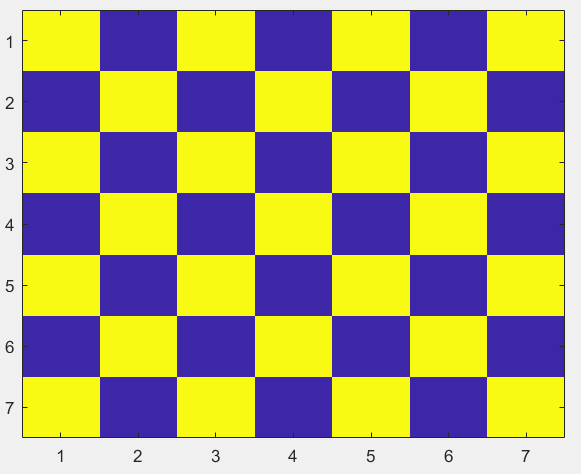
\includegraphics[width=0.7\linewidth]{G_nullSpaceVectors}
	\caption{Imagesc representing the kernel of G}
	\label{fig:gnullspacevectors}
\end{figure}

Since we make use of wavefront prediction in our models, if we see the above pattern as the predicted wavefront, we can be cautious and change the input ($\phi_{DM}$) so as to move away from the wavefront that would otherwise cause the slope vector to be falsely 0.

\subsubsection*{Question 4}


\subsubsection*{Question 5}
The control law we derived in Section 1 is represented by equation \ref{eq:delta_uk}, in which we calculate the input to be applied at a time instant based on the slope measurement at that time instant and the previous input.

It is a recursive relation, and we assume that at the first time instant, we do not apply any control input. Based on this, we calculate the control input ($\phi_{DM}(k)$) for the rest of the time instants based on the control law represented by equation (6) in the assignment (on which equation \ref{eq:delta_uk}'s derivation is based).

We see that in

\begin{equation*}
\hat\delta u(k) = (H^{T}H)^{-1}H^{T}C_{\phi}(0)G^{T}(GC_{\phi}(0)G^{T} + \sigma_{e}^{2}I)^{-1}s(k)
\end{equation*}

there is a mix of online and offline computations, as listed below:

\begin{itemize}
	\item say, V = $ (H^{T}H)^{-1}H^{T}C_{\phi}(0)G^{T}(GC_{\phi}(0)G^{T} + \sigma_{e}^{2}I)^{-1}$. We know that V can be computed offline since its value does not depend on any sample instant k (the H, $C_{\phi}(0)$ and G matrices do depend on the sensor array size, but since the above computation needs to be done only once, there's no exponential increase in the number of computations with increasing loop size)
	\item Multiplying V with s(k) cannot be done offline since it depends on the slope vector s(k) at time instant k, and the number of computations grows quadratically with increasing sensor array size (since there is a squaring term involved).
	\item Likewise, the number of computations for calculating u(k) from u(k-1) grows quadratically with the increasing actuator array size. Since it is a recursive relation, it cannot be done offline.
\end{itemize}

Per iteration, there are $2p^{2}x m^2$ elementary multiplication operations and $(2p^{2} - 1)x m^2$ elementary addition operations from the V*s(k) matrix multiplication, and a further $m^2$ elementary addition operations from adding the product to u(k-1).

Hence, we have a total of $2p^{2}x m^2$ multiplication and $2p^{2}x m^2$ addition operations as online computations.

Thus, we can conclude that this method is not very scalable purely in terms of the sensor and actuator array sizes involved, since with large array sizes, the number of computations per iteration grows quadratically ($\mathcal{O}(n^2)$).

%----------------------------------------------- --------------------------------
% REFERENCES
%-------------------------------------------------------------------------------
\newpage
\section*{References}
\addcontentsline{toc}{section}{References}


M. Verhaegen, V. Verdult. "Filtering and System Identification: A Least-Squares Approach", Cambridge University Press, 2007.

\section*{Appendix}

Please find henceforth all MATLAB code associated with this assignment.

\end{document}

%-------------------------------------------------------------------------------
% SNIPPETS
%-------------------------------------------------------------------------------

%\begin{figure}[!ht]
%	\centering
%	\includegraphics[width=0.8\textwidth]{file_name}
%	\caption{}
%	\centering
%	\label{label:file_name}
%\end{figure}

%\begin{figure}[!ht]
%	\centering
%	\includegraphics[width=0.8\textwidth]{graph}
%	\caption{Blood pressure ranges and associated level of hypertension (American Heart Association, 2013).}
%	\centering
%	\label{label:graph}
%\end{figure}

%\begin{wrapfigure}{r}{0.30\textwidth}
%	\vspace{-40pt}
%	\begin{center}
%		\includegraphics[width=0.29\textwidth]{file_name}
%	\end{center}
%	\vspace{-20pt}
%	\caption{}
%	\label{label:file_name}
%\end{wrapfigure}

%\begin{wrapfigure}{r}{0.45\textwidth}
%	\begin{center}
%		\includegraphics[width=0.29\textwidth]{manometer}
%	\end{center}
%	\caption{Aneroid sphygmomanometer with stethoscope (Medicalexpo, 2012).}
%	\label{label:manometer}
%\end{wrapfigure}

%\begin{table}[!ht]\footnotesize
%	\centering
%	\begin{tabular}{cccccc}
%	\toprule
%	\multicolumn{2}{c} {Pearson's correlation test} & \multicolumn{4}{c} {Independent t-test} \\
%	\midrule	
%	\multicolumn{2}{c} {Gender} & \multicolumn{2}{c} {Activity level} & \multicolumn{2}{c} {Gender} \\
%	\midrule
%	Males & Females & 1st level & 6th level & Males & Females \\
%	\midrule
%	\multicolumn{2}{c} {BMI vs. SP} & \multicolumn{2}{c} {Systolic pressure} & \multicolumn{2}{c} {Systolic Pressure} \\
%	\multicolumn{2}{c} {BMI vs. DP} & \multicolumn{2}{c} {Diastolic pressure} & \multicolumn{2}{c} {Diastolic pressure} \\
%	\multicolumn{2}{c} {BMI vs. MAP} & \multicolumn{2}{c} {MAP} & \multicolumn{2}{c} {MAP} \\
%	\multicolumn{2}{c} {W:H ratio vs. SP} & \multicolumn{2}{c} {BMI} & \multicolumn{2}{c} {BMI} \\
%	\multicolumn{2}{c} {W:H ratio vs. DP} & \multicolumn{2}{c} {W:H ratio} & \multicolumn{2}{c} {W:H ratio} \\
%	\multicolumn{2}{c} {W:H ratio vs. MAP} & \multicolumn{2}{c} {\% Body fat} & \multicolumn{2}{c} {\% Body fat} \\
%	\multicolumn{2}{c} {} & \multicolumn{2}{c} {Height} & \multicolumn{2}{c} {Height} \\
%	\multicolumn{2}{c} {} & \multicolumn{2}{c} {Weight} & \multicolumn{2}{c} {Weight} \\
%	\multicolumn{2}{c} {} & \multicolumn{2}{c} {Heart rate} & \multicolumn{2}{c} {Heart rate} \\
%	\bottomrule
%	\end{tabular}
%	\caption{Parameters that were analysed and related statistical test performed for current study. BMI - body mass index; SP - systolic pressure; DP - diastolic pressure; MAP - mean arterial pressure; W:H ratio - waist to hip ratio.}
%	\label{label:tests}
%\end{table}